% !TEX root = ../my-thesis.tex
%
\chapter{Search for dark matter in association with a dark Higgs boson decaying to a pair of weak vector bosons}
\label{ch:monoSVV}

\section{Introduction}
\label{sec:monoSVV:introduction}
This chapter describes the search for dark matter in association with a dark Higgs boson \(s\) decaying to a pair of weak vector bosons, which is referred to as the \(\met + \sVV\) search. The results presented in this chapter complement those presented in \Cref{ch:monoSbb} by extending the dark Higgs boson mass reach.

The \(\met + \sVV\) signature is explored by a search in the fully hadronic channel, as the hadronic decays of weak vector bosons have the largest branching fraction~\cite{Tanabashi2018}. The search makes use of the full ATLAS Run-2 \HepProcess{\Pp\Pp} dataset, corresponding to an integrated luminosity of \SI{139}{\per\femto\barn}.

The \(\met + \sVV\) search investigates the yet uncharted signature of missing transverse momentum and the resonant production of a pair of hadronically decaying weak vector bosons, whose decays give rise to a system of up to four jets.
The challenging event topology is addressed with the novel reconstruction technique of the Track-Assisted-Reclustering (TAR) jet algorithm~\cite{ATL-PHYS-PUB-2018-012}, which enables the reconstruction of large-radius jets from calibrated small-radius jets and ID tracks.
The results of this search have been presented in Ref.~\cite{ATLAS-CONF-2020-036}.

\Cref{sec:monoSVV:physics} introduces the signal and background processes in the \(\met + \sVV\) search. The analysis strategy is outlined in \Cref{sec:monoSVV:analysis}. The corresponding object and event selection, including the definition of the signal region is described in \Cref{sec:monoSVV:selection}, whereas the background estimation strategy and the definitions of the control regions are described in \Cref{sec:monoSVV:backgrounds}.
The systematic uncertainties taken into account in the statistical model are described in \Cref{sec:monoSVV:systematics}, while the statistical model itself is provided in \Cref{sec:monoSVV:model}. The observed results are presented and discussed in \Cref{sec:monoSVV:results}. A conclusion is given in \Cref{sec:monoSVV:conclusion}.

\section{Signal and background processes}
\label{sec:monoSVV:physics}
The analysis investigates dark matter production in the framework of the 2MDM simplified model, using the configuration which is described in \Cref{sec:monoSbb:physics:2mdm}. The background processes are outlined in \Cref{sec:monoSVV:physics:backgrounds}. The simulated signal and background samples are summarised in \Cref{sec:monoSVV:physics:mcsamples}.

\subsection{Background processes}
\label{sec:monoSVV:physics:backgrounds}
The dominant background processes resulting in the signature of two weak vector bosons and substantial \met are \zjets production (\SI{61}{\percent} background contribution) and \wjets production (\SI{32}{\percent} background contribution).
Sub-dominant background processes include \ttbar production, \HepProcess{\PW \PW}, \HepProcess{\PW \PZ}, and \HepProcess{\PZ \PZ} diboson production, single top quark production, SM \VHbb production, and multijet events.

The dominant background processes are estimated using simulated samples, whose normalisation is constrained by control region data. The smaller background processes are estimated purely by simulation. The multijet background is estimated to be negligible based on a data-driven estimate.


\subsection{Simulated Monte Carlo samples}
\label{sec:monoSVV:physics:mcsamples}
The signal and background processes with the MC event generators, parton shower models and PDF sets used for their description are summarised in \Cref{tab:monoSVV:physics:mcsamples:generators}. Detailed descriptions of the background samples are provided in \Cref{sec:common:data:mc}.

The signal process in the 2MDM simplified model is simulated on grids defined by the mediator mass \mZp and the dark Higgs boson mass \ms for a fixed dark matter particle mass \(\mchi = \SI{200}{\giga\electronvolt}\).
The signals are simulated by scanning the mass of the dark Higgs boson \ms in the range \SIrange{160}{360}{\giga\electronvolt} in \SI{25}{\giga\electronvolt} steps considering \PZprime boson masses of \SI{0.5}{\tera\electronvolt}, \SI{1}{\tera\electronvolt}, \SI{1.7}{\tera\electronvolt}, and \SI{2.1}{\tera\electronvolt}.

The coverage in the \mZp-\ms plane of the parameter space is extended by an interpolation procedure. The interpolation is based on reweighting the simulated samples to signal configurations with different \mZp using events generated at particle level neglecting detector effects~\cite{Rogozhnikov2016}. The interpolation procedure provides the exclusion contour with a \(\Delta \mZp = \SI{100}{\giga\electronvolt}\) spacing.

The simulated events are generated at leading-order (\LO) accuracy with the \MGMCatNLOV{2.6.2} event generator~\cite{Alwall:2014hca} interfaced to the \PYTHIAV{8.230}~\cite{Sjostrand:2014zea} parton shower and hadronisation model, using the \textsc{NNPDF23} PDF set~\cite{Ball:2012cx} and the \AFourteen set of tuned parameters~\cite{ATL-PHYS-PUB-2014-021}.
To remove the overlap between the hard scattering and the parton shower model, the CKKW-L merging procedure~\cite{Lnnblad2002,Lnnblad2012} is applied with the matching scale set to \SI{40}{\giga\electronvolt}.

\begin{table}[htbp]
\caption{List of the signal and background processes with the MC event generators, sets of PDFs and tunes used for their description in the \(\met + \sVV\) search.}
\label{tab:monoSVV:physics:mcsamples:generators}
\centering
\resizebox{1.\textwidth}{!}{%
\begin{tabular}{l l l}
\toprule
Process & Generator & PDF / parton shower tune \\
\midrule
\textbf{Signal}  & & \\
2MDM             & \MGMCatNLOV{2.6.2} & \textsc{NNPDF23LO} / \AFourteen \\
simplified model & + \PYTHIAV{8.230} & \\
\midrule
\textbf{Top quark}   & & \\
\ttbar               & \POWHEGBOXV{2} + \PYTHIAV{8.230} & \textsc{NNPDF30NLO} / \AFourteen \\
\Pqt (\(s\)-channel) & \POWHEGBOXV{2} + \PYTHIAV{8.230} & \textsc{NNPDF30NLO} / \AFourteen \\
\Pqt (\(t\)-channel) & \POWHEGBOXV{2} + \PYTHIAV{8.230} & \textsc{NNPDF30NLO} / \AFourteen \\
\Pqt (\(\PW t\))     & \POWHEGBOXV{2} + \PYTHIAV{8.230} & \textsc{NNPDF30NLO} / \AFourteen \\
\midrule
\textbf{\(V\) + jets} & & \\
\Wjets & \SHERPAV{2.2.1} & \textsc{NNPDF30NNLO} / \SHERPA-tune \\
\Zjets & \SHERPAV{2.2.1} & \textsc{NNPDF30NNLO} / \SHERPA-tune \\
\midrule
\textbf{Diboson}    & & \\
\HepProcess{\PW\PW} & \SHERPAV{2.2.1}                  & \textsc{NNPDF30NLO} / \SHERPA-tune \\
\HepProcess{\PW\PZ} & \SHERPAV{2.2.1}                  & \textsc{NNPDF30NLO} / \SHERPA-tune \\
\HepProcess{\PZ\PZ} & \SHERPAV{2.2.1}                  & \textsc{NNPDF30NLO} / \SHERPA-tune \\
\VHbb               & \POWHEGBOXV{2} + \PYTHIAV{8.212} & \textsc{NNPDF30NLO} / \AZNLO \\
\bottomrule
\end{tabular}%
}
\end{table}


\section{Analysis strategy}
\label{sec:monoSVV:analysis}
The signature of dark matter particle production in association with a dark Higgs boson \(s\) decaying to pairs of weak vector bosons in the hadronic decay channel is provided by missing transverse momentum \met recoiling against a system of up to four jets resulting from the \HepProcess{s \to V(\Pq\Pq) V(\Pq\Pq)} decay.

The signal region (SR) is defined by the requirement of substantial missing transverse momentum and a dark Higgs boson candidate.
The sensitivity of the search is optimised over a broad range of dark Higgs boson candidate momenta by considering two event topologies for the dark Higgs boson candidate reconstruction.

In events with a highly boosted dark Higgs boson candidate, the dark Higgs boson decay products become collimated and can be fully captured within a single TAR jet. This event topology is referred to as the merged category.

Moderately boosted dark Higgs boson candidates result in less collimated decay products, which might be captured only partially by a single TAR jet. Therefore, a dedicated algorithm is employed to reconstruct dark Higgs boson candidates from TAR jets augmented with one or two small-radius jets. This event topology is referred to as the intermediate category.

In contrast to the other searches discussed in this dissertation, no resolved category is considered, as the sensitivity in the \(\met + \sVV\) signature is driven by highly boosted boson decays.

Potential ambiguities in the selection are resolved by giving preference to the merged category, which has better sensitivity. \Cref{fig:monoSVV:physics:topologies} illustrates the two event topologies in the transverse plane of the detector.

\begin{figure}[htbp]
    \centering
    \begin{subfigure}{0.45\textwidth}
      \centering
      \includegraphics[width=0.95\textwidth]{figures/monoS/signature_tarmerged.pdf}
    \end{subfigure}
    \hfill
    \begin{subfigure}{0.45\textwidth}
      \centering
      \includegraphics[width=0.95\textwidth]{figures/monoS/signature_intermediate.pdf}
    \end{subfigure}
    \caption{Illustrations of the merged and intermediate event topologies in the \(\met + \sVV\) search.}
    \label{fig:monoSVV:physics:topologies}
\end{figure}

Additional requirements on kinematic properties and the event topology further increase the sensitivity of the search. The primary discriminating variable in the statistical analysis is the invariant mass of the dark Higgs boson candidate. Moreover, the merged category SR is further classified in the two \met bins \SIrange{300}{500}{\giga\electronvolt} and \SI{500}{\giga\electronvolt} or more to benefit from the increased signal sensitivity with higher \met.

The SR selection vetoes events containing electrons or muons. The control regions (CRs) require the presence of either one muon (1 muon CR) or two electrons or muons (2 lepton CR). As SR and CRs have different requirements on the lepton multiplicity, they do not overlap. Similar to the \(\met + \Hbb\) search, the CR selections do not employ \met but instead the \metnomu variable in the 1 muon CR and the transverse momentum of the dilepton system \ptll in the 2 lepton CR.

The SR and CRs considered in the analysis are
\begin{itemize}
	\item 0 lepton SR with no electrons and no muons, including the \merged category with two \met bins and the intermediate category,
	\item 1 muon CR with one muon and no electrons, including the merged category with two \metnomu bins and the intermediate category,
	\item 2 lepton CR with two same-flavour leptons, including the merged category with two \ptll bins and the intermediate category,
\end{itemize}

A graphical overview of all regions and categories considered in the analysis with their relative background composition is given in \Cref{fig:monoSVV:analysis:overview}.
\begin{figure}[htbp]
	\centering
	\includegraphics[width=1.\textwidth]{figures/monoS/monoSoverview.pdf}
	\caption{Overview of all regions and categories considered in the \(\met + \sVV\) search with their relative background composition. Each region is composed of the merged event topology category and the intermediate event topology category. The merged category is further divided in two \ptv bins, where \ptv denotes \met in the signal region, \metnomu in the 1 muon CR, and \ptll in the 2 lepton CR, respectively.}
	\label{fig:monoSVV:analysis:overview}
\end{figure}


\section{Object and event selection}
\label{sec:monoSVV:selection}
The selection requirements for events considered in the signal region are outlined below. The specific choices for physics object definitions are summarised in \Cref{sec:monoSVV:selection:objects}.
The common baseline selection used in the SR and CRs is described in \Cref{sec:monoSVV:selection:baseline}, while the SR event selection is described in \Cref{sec:monoSVV:selection:sr}.

\subsection{Object selection}
\label{sec:monoSVV:selection:objects}
The physical objects used in the \(\met + \sVV\) search are based on the object definitions, which are introduced in \Cref{sec:common:objects}.

The novel TAR jet algorithm is exploited to reconstruct the dark Higgs boson candidates.
The TAR jet algorithm provides superior jet substructure resolution even in dense event topologies by supplementing reclustered jets with precision tracking information.
The steps involved in the reconstruction of TAR jets are shown in \Cref{fig:monoSVV:selection:objects:tar-algorithm}.

\begin{figure}[htbp]
  \centering
  \includegraphics[width=1.0\textwidth]{figures/monoS/tar_algorithm.pdf}
  \caption{Flowchart illustrating the TAR jet algorithm. The input objects to the algorithm are shown in blue boxes. Figure adapted from Ref.~\cite{ATL-PHYS-PUB-2018-012}.}
  \label{fig:monoSVV:selection:objects:tar-algorithm}
\end{figure}

\begin{enumerate}
  \item \textbf{Jet reclustering.} The calibrated small-radius jets are used as inputs to the \antikt algorithm with radius parameter \(R=0.8\). The resulting jets with large-radius parameter are processed with the trimming algorithm (c.f. \Cref{sec:methods:event-reconstruction:jets:larger}) using the parameters \(f_{\text{cut}} = 0.05\) and \(R_{\text{sub}} = 0.2\) to remove sub-jets originating from pile-up.
  \item \textbf{Track matching.} The ID tracks are matched to the reclustered jet's constituent small-radius jets. This is done using first the ghost-association technique (c.f. \Cref{sec:methods:event-reconstruction:jets:trackjets}) and then matching the remaining not yet associated tracks to the small-radius jets within \(\Delta R(\text{sub-jet}, \text{track}) = \sqrt{\Delta \eta^2 + \Delta \varphi^2} = 0.5\).
  \item \textbf{Scaling of track transverse momenta.} As the ID is only sensitive to charged particles, the track momenta need to be corrected for the presence of neutral hadrons in the jet. Consequently, the transverse momenta of the constituent tracks of the small-radius jets are scaled with a correction factor, which is defined as the ratio of the \pt of the small-radius jet to which the tracks were matched over the sum of all its constituent tracks. As a result, the scaled track transverse momenta are
  \begin{align}
      \pt^{\text{track, new}} = \frac{\pt^{\text{track}}}{\sum_{\text{tracks in jet}} \pt^{\text{track}}} \times \pt^{\text{jet}}.
  \end{align}
  \item \textbf{Jet substructure from tracking information.} The TAR jet mass \mtar and jet substructure observables are computed using the re-scaled constituent tracks of the TAR jet.
\end{enumerate}

The major advantage of the TAR jet algorithm is the improved jet mass and substructure resolution, which is demonstrated in \Cref{fig:monoSVV:selection:objects:tar-resolution}. Considering event topologies with hadronically decaying \PW bosons, the resolution of the jet mass and the \dtwo energy correlation ratio (c.f. \Cref{eq:monoV:selection:sr:dtwo}) computed with TAR jets is compared against conventional large-radius jets (c.f. \Cref{sec:methods:event-reconstruction:jets:larger}).
The best resolution for \mtar is achieved for jets with \(\pt < \SI{800}{\giga\electronvolt}\) with relative gains with respect to conventional large-radius jets of up to \SI{35}{\percent}. Also for the high-\pt regime \(\pt > \SI{1500}{\giga\electronvolt}\), TAR jets have the best performance. Similarly, the \dtwo resolution achieved with TAR jets provides a relative gain of \SI{50}{\percent} over the conventional large-radius jet substructure and deteriorates more slowly with increasing jet \pt.

\begin{figure}[hbtp]
  \centering
  \begin{subfigure}{1.\textwidth}
    \centering
  \includegraphics[width=0.9\textwidth]{figures/monoS/tar_massresolution.pdf}
    \caption{Jet mass resolution}
  \end{subfigure}
  \\
  \begin{subfigure}{1.\textwidth}
    \centering
    \includegraphics[width=0.9\textwidth]{figures/monoS/tar_d2resolution.pdf}
    \caption{\dtwo energy correlation ratio resolution}
  \end{subfigure}
  \caption{Jet mass resolution (top) and \dtwo energy correlation ratio resolution (bottom) in simulated events with hadronically decaying \PW bosons. The resolution of TAR jet observables is compared to that of conventional large-radius jets. Figures adapted from Ref.~\cite{ATL-PHYS-PUB-2018-012}.}
  \label{fig:monoSVV:selection:objects:tar-resolution}
\end{figure}

Furthermore, the algorithm provides flexibility in the jet definition by using already calibrated objects as inputs to the jet reclustering. The propagation of the small-radius jet and tracking uncertainties allows avoiding a dedicated TAR jet calibration, as the TAR jet uncertainties can be derived from its constituent objects.

The TAR jets employed in this search have to satisfy \(\pt > \SI{100}{\giga\electronvolt}\) and \(\abs{\eta} < 2.0\).
The TAR jet definition is summarised in \Cref{tab:monoSVV:selection:objects:tarjets}.

\begin{table}[hbtp]
\caption{TAR jet definition in the \(\met + \sVV\) search}
\label{tab:monoSVV:selection:objects:tarjets}
\centering
\begin{tabular}{l l}
\toprule
 & TAR jets \\
\midrule
Jet algorithm & \antikt        \\
\(R\)-parameter & \num{0.8}    \\
Grooming algorithm & trimming  \\
\(R_{\text{sub}}\) & \num{0.2} \\
\(f_{cut}\) & \num{0.05}       \\
\multirow{2}{*}{Input constituents} & small-radius jets      \\
                                    & and ID tracks          \\
\(\Delta R(\text{sub-jet}, \text{track})\) & \num{0.5}       \\
Pseudorapidity range & \(\abs{\eta} < 2.0\)                  \\
Transverse momentum & \(\pt > \SI{100}{\giga\electronvolt}\) \\
\bottomrule
\end{tabular}
\end{table}

The contributions of background processes are suppressed further by additional requirements on small-radius jets.
Variable radius (VR) track jets are used to identify \bjets using the MV2 discriminant with a fixed-cut working point corresponding to a \btagging efficiency of \SI{77}{\percent}.

The lepton definitions are the same as those used in the \(\met + \Hbb\) search (c.f. \Cref{sec:monoH:selection:objects}).

The missing transverse momentum \met is reconstructed from the calibrated physics objects in the event and the track-based soft term (TST) using the \textsc{Tight} working point due to the increased pile-up in the 2017--2018 data-taking.
In the CRs, the \metnomu and \ptll substitute observables are used, which describe how background processes are contributing to the signal region. Their definition is the same as in the \(\met + \Hbb\) search (c.f. \Cref{sec:monoH:selection:objects}).
The object-based \met significance is used to suppress events with fake \met caused by resolution effects.

Potential ambiguities in the reconstruction, such as reconstructed objects matching multiple object hypotheses, must be resolved by an overlap removal procedure. The overlap removal procedure is identical to that described in \Cref{sec:monoH:selection:objects} except for the overlap removal step for large-radius jets and electrons, which is not applied.


\subsection{Baseline selection}
\label{sec:monoSVV:selection:baseline}
The SR and CR definition is based on a common baseline selection and common requirements to suppress the multijet background. These selection requirements share similarities with those employed in the \(\met + \Vqq\) and \(\met + \Hbb\) searches, which are presented in \Cref{sec:monoV:selection:baseline}, \Cref{sec:monoV:selection:antiqcd}, and \Cref{sec:monoH:selection:baseline}.

In addition to the requirements on data quality, vertex reconstruction, jet cleaning, and the trigger, which are the same as in the \(\met + \Hbb\) search, vetoes on events containing \btagged VR track jets or baseline tau lepton candidates are applied to reduce the background contribution of \ttbar and \Vjets processes.

Selected events in the SR have to satisfy \(\met > \SI{200}{\giga\electronvolt}\), thereby ensuring operation in the region of full \met trigger efficiency and avoiding the need for an \met trigger calibration.

The multijet background is suppressed by applying two multijet-suppression requirements.
\begin{itemize}
  \item Selected events have to pass a requirement on the minimum azimuthal distance between the three highest-\pt central jets \(\min \Delta \varphi(\text{jets}_{1,2,3}, \met) > \SI{20}{\degree}\).
  \item Selected events also have to satisfy a requirement on the object-based \met significance \(\mathcal{S} > 15\) in the SR. In the 1 muon CR, the requirement is based on a modified object-based \met significance \(\mathcal{S}^{\text{no }\mu}\), neglecting the highest-\pt muon in the \met reconstruction.
\end{itemize}

Similarly to the \(\met + \Hbb\) search, the multijet-suppression requirements are not applied in the 2 lepton CR to increase the statistical precision of the CR. The requirement of 2 leptons already strongly suppresses potential contamination through multijet processes. Instead, a requirement on the object-based \met significance \(\mathcal{S} < 15\) is applied to reject potential signal processes with a \(\met + \HepProcess{s \to Z(\Pl\Pl)V(\Pq\Pq)}\) signature.

The baseline selection requirements are summarised in \Cref{tab:monoSVV:selection:baseline:summary}.

\begin{table}[hbtp]
\caption{List of the baseline selection requirements employed in the \(\met + \sVV\) search.}
\label{tab:monoSVV:selection:baseline:summary}
\centering
\resizebox{1.\textwidth}{!}{%
\begin{tabular}{l lll}
\toprule
Baseline selection & \textbf{0 lepton SR} & \textbf{1 muon CR} & \textbf{2 lepton CR} \\
\midrule
Data quality & \multicolumn{3}{c}{basic requirements vetoing corrupted data or incomplete events} \\
Vertex reconstruction & \multicolumn{3}{c}{primary vertex with at least two associated tracks} \\
Jet cleaning & \multicolumn{3}{c}{veto on events containing jets flagged as \textsc{BadLoose} jets} \\
Trigger & \met trigger & \met trigger & single lepton trigger \\
\midrule
\bjet veto & \multicolumn{3}{c}{0 \btagged VR track jets in the event} \\
Tau lepton veto & \multicolumn{3}{c}{0 baseline tau lepton candidates in the event} \\
Missing transverse momentum & \(\met > \SI{200}{\giga\electronvolt}\) & \(\metnomu > \SI{200}{\giga\electronvolt}\) & \(\ptll > \SI{200}{\giga\electronvolt}\) \\
\midrule
\multirow{2}{*}{Multijet suppression} & \(\min \Delta \varphi(\text{jets}_{1,2,3}, \met) > \SI{20}{\degree}\) & \(\min \Delta \varphi(\text{jets}_{1,2,3}, \metnomu) > \SI{20}{\degree}\) & no \\
& \met significance \(\mathcal{S} > 15\) & \metnomu significance \(\mathcal{S}^{\text{no }\mu} > 15\) & no \\
\midrule
Signal suppression & no & no & \met significance \(\mathcal{S} < 15\) \\
\bottomrule
\end{tabular}%
}
\end{table}


\subsection{Signal region selection}
\label{sec:monoSVV:selection:sr}
The SR event selection employs a veto on events containing baseline electrons or baseline muons, as the \(\met + \sVV\) search targets the hadronic decay mode of the weak vector bosons \(V\). Two complementary selection categories are considered to cover the merged and intermediate event topologies, with priority given to the merged category in case of ambiguities.

The events comprising the \textbf{merged category} are selected by applying the baseline selections and requiring \(\met > \SI{300}{\giga\electronvolt}\). The dark Higgs boson candidate in the merged category is reconstructed using the TAR jet with the highest transverse momentum. The dark Higgs boson candidate \pt is strongly correlated with \met. Therefore, its transverse momentum is required to be larger than \SI{300}{\giga\electronvolt} as well.

The TAR jet substructure is used to identify the four-prong dark Higgs boson decay.
To this end, the set of \(N\)-subjettiness~\cite{Thaler2011,Thaler2012} jet substructure observables, denoted \(\tau_{N}\), is employed. \(N\)-subjettiness allows quantifying how well jets can be described as containing \(N\) or fewer sub-jets.

The calculation of \(\tau_{N}\) begins with the definition of \(N\) sub-jet axes within the TAR jet by using the exclusive \(k_{\text{T}}\) clustering algorithm, which reconstructs jets by approximately inverting the QCD parton shower evolution and continues with the jet reconstruction until a desired number of jets is found.
The \(N\)-subjettiness is calculated via
\begin{align}
    \tau_{0} &= \sum_{k} p_{\text{T}, k} \times R_{0}, \\
    \tau_{N} &= \frac{1}{\tau_{0}} \times \left(\sum_{k} p_{\text{T}, k} \times R_{k}^{\text{min}}\right),
\end{align}
where \(R_{0} = 0.8\) is radius of the TAR jet, \(k\) runs over the constituent tracks in a given TAR jet, \(p_{\text{T}, k}\) are their transverse momenta, and \(R_{k}^{\text{min}}\) is the distance in the rapidity-azimuth plane between the constituent track \(k\) and the axis of the closest sub-jet.

In this search, the winner-takes-all scheme~\cite{Bertolini2014,Larkoski2014} is employed, in which the sub-jet axis is taken to be parallel with the momentum of the hardest sub-jet constituent, as it provides increased discrimination power.

Small values of \taufourtwo and \taufourthree correspond to TAR jets with signal-like four-prong substructure, whereas large values indicate the jets originating from background processes.

Therefore, the \(N\)-subjettiness ratios \(\taufourtwo = \tau_{4} / \tau_{2}\) and \(\taufourthree = \tau_{4} / \tau_{3}\) provide strong discrimination of four-prong decays against two- or three-prong decays.
The dark Higgs boson candidate TAR jet is required to satisfy the requirements on the \(N\)-subjettiness ratios \(0 < \taufourtwo < 0.3\) and \(0 < \taufourthree < 0.6\). The distributions of the \(N\)-subjettiness ratios for signal and background processes are shown in \Cref{fig:monoSVV:selection:sr:substructure-1d}.

\begin{figure}[hbtp]
  \centering
  \begin{subfigure}{1.\textwidth}
    \centering
    \includegraphics[width=.95\textwidth]{figures/monoS/monoS_SR_Merged_Tau42.pdf}
    \caption{\taufourtwo distribution of the highest-\pt TAR jet}
  \end{subfigure}
  \\
  \begin{subfigure}{1.\textwidth}
    \centering
  \includegraphics[width=.95\textwidth]{figures/monoS/monoS_SR_Merged_Tau43.pdf}
    \caption{\taufourthree distribution of the highest-\pt TAR jet}
  \end{subfigure}
  \caption{Dark Higgs boson candidate TAR jet substructure variables \taufourtwo (top) and \taufourthree (bottom) for two \(\met + \sVV\) signal processes with \(\mZp = \SI{1}{\tera\electronvolt}\) and \(\ms = \SI{160}{\giga\electronvolt}\) or \SI{235}{\giga\electronvolt} and background processes. The simulated background processes are normalised to the theoretical prediction. The requirements on the SR merged category event selection are applied, except for the requirement on the variable which is shown. The cut value is indicated by a long-dashed line.}
  \label{fig:monoSVV:selection:sr:substructure-1d}
  % python XAMPPplotting/python/MCPlots.py -c XAMPPmonoS/data/PlottingConfigs/DSConfigs/MonoS_CC_SR.py --noATLAS --noSyst --noSignalStack -r SR_Merged_noTau42 -v cand_scalar_tarjets8_notau42cut_tau42 --LegendTextSize 20 --LegendXCoords 0.57 0.97 --LegendYCoords 0.45 0.925 -l 139 --noRatio  --EntriesPerLegendColumn 12
  % python XAMPPplotting/python/MCPlots.py -c XAMPPmonoS/data/PlottingConfigs/DSConfigs/MonoS_CC_SR.py --noATLAS --noSyst --noSignalStack -r SR_Merged_noTau43 -v cand_scalar_tarjets8_notau43cut_tau43 --LegendTextSize 20 --LegendXCoords 0.20 0.7 --LegendYCoords 0.5 0.775 -l 139 --noRatio  --EntriesPerLegendColumn 3
\end{figure}

As the jets are more collimated for signals with lower \ms, the corresponding \taufourtwo and \taufourthree distributions accumulate at lower values than for signals with larger \ms.

\Cref{fig:monoSVV:selection:sr:substructure-2d} shows correlations between the dark Higgs boson candidate mass \(m_{VV}\) and the \(N\)-subjettiness ratio variables for a representative signal process with \(\mZp = \SI{1.7}{\tera\electronvolt}\) and \(\ms = \SI{160}{\giga\electronvolt}\), depending on the number of partons matched to the TAR jet using the \(\Delta R\) distance measure.

The dark Higgs boson candidate mass is reconstructed deficiently if not all four partons are contained within the TAR jet. Therefore, the tight requirements on the jet substructure variables \taufourtwo and \taufourthree not only provide discrimination against background processes but also improve the signal reconstruction by restricting the merged selection to events in which the full dark Higgs decay is most likely contained in the TAR jet.

\begin{figure}[hbtp]
  \centering
  \begin{subfigure}{.49\textwidth}
    \centering
    \includegraphics[width=1.\textwidth]{figures/monoS/truthMerged/mzp1700ms160/sVVmerged_truth_lt4matchedquarks_mVStau42.pdf}
    \caption{\taufourtwo, less than four matched partons}
  \end{subfigure}
  \begin{subfigure}{.49\textwidth}
    \centering
  \includegraphics[width=1.\textwidth]{figures/monoS/truthMerged/mzp1700ms160/sVVmerged_truth_4matchedquarks_mVStau42.pdf}
    \caption{\taufourtwo, four matched partons}
  \end{subfigure}
  \\
  \begin{subfigure}{.49\textwidth}
    \centering
    \includegraphics[width=1.\textwidth]{figures/monoS/truthMerged/mzp1700ms160/sVVmerged_truth_lt4matchedquarks_mVStau43.pdf}
    \caption{\taufourthree, less than four matched partons}
  \end{subfigure}
  \begin{subfigure}{.49\textwidth}
    \centering
  \includegraphics[width=1.\textwidth]{figures/monoS/truthMerged/mzp1700ms160/sVVmerged_truth_4matchedquarks_mVStau43.pdf}
    \caption{\taufourthree, four matched partons}
  \end{subfigure}
  \caption{Correlation between the dark Higgs boson candidate mass \(m_{VV}\) and the \(N\)-subjettiness ratio variables \taufourtwo (top) and \taufourthree (bottom). The distributions are shown separately for events in which not all four partons are contained within the dark Higgs boson candidate TAR jet (left) and events in which all four partons are contained (right). The cut value used in the substructure requirements is indicated by a dashed line.}
  \label{fig:monoSVV:selection:sr:substructure-2d}
\end{figure}

The invariant mass of the TAR jet, denoted \(m_{VV}\), is used as the primary discriminating variable in the statistical analysis. Additionally, the merged event selection considers two \met bins.


The event selection of the \textbf{intermediate category} is optimised for events with moderate amount of missing transverse momentum \(\met > \SI{200}{\giga\electronvolt}\), which are not selected in the merged category.
The resulting event topology consists of one highly boosted weak vector boson whose decay products are contained within a single TAR jet and another weak vector boson whose smaller boost enables the reconstruction of its decay products with small-radius jets. The intermediate category selection is particularly relevant for signal processes with large \ms, as the separation of the weak vector bosons increases with it.

A dedicated algorithm is developed to address this scenario, which exploits both the TAR jet mass and the TAR jet substructure to identify weak vector boson candidates. As \PW and \PZ bosons are almost indistinguishable given the coarse jet mass resolution \(\sigma(m)> \abs{\mW - \mZ}\), the algorithm employs the \PW boson mass to define weak vector boson candidates. Choosing the \PW boson mass instead of the \PZ boson mass is favourable because of the larger branching fraction for the dark Higgs boson decay to \PW bosons as opposed to \PZ bosons.

The so-called \textsc{TAR+comb} algorithm is described below.

% is illustrated in \Cref{fig:monoSVV:selection:sr:tarcomb} and
% \begin{figure}[hbtp]
%   \centering
%   \includegraphics[width=1.\textwidth]{figures/monoS/TARcomb.pdf}
%   \caption{Flowchart of the \textsc{TAR+comb} algorithm for the reconstruction of dark Higgs boson candidates in the intermediate event topology.}
%   \label{fig:monoSVV:selection:sr:tarcomb}
% \end{figure}

\begin{enumerate}
  \item \textbf{Decision based on TAR jet}. The highest-\pt TAR jet is considered. If its mass \mtar is in the range \SIrange{60}{100}{\giga\electronvolt} and the energy correlation ratio \dtwo computed with TAR jet substructure satisfies \(\dtwo < 1.5\), the TAR jet is considered as a weak vector boson candidate and the second weak vector boson candidate is reconstructed with small-radius jets. Otherwise, if \(\mtar > \SI{100}{\giga\electronvolt}\), the majority of the dark Higgs decay is contained within the TAR jet and it is considered as an ``incomplete'' dark Higgs boson candidate and the missing components of the dark Higgs boson candidate are supplemented by small-radius jets.
  \item[2.1] \textbf{Case 1: weak vector boson candidate}, \(\SI{60}{\giga\electronvolt} < \mtar < \SI{100}{\giga\electronvolt}\).
  \begin{itemize}
    \item The small-radius jets within \(\Delta R < 2.5\) of the weak vector boson candidate are considered unless they overlap with it based on the \(\Delta R\) distance measure.
    \item All possible combinations of small-radius jet pairs are formed and ordered by the difference of their invariant mass to the \PW boson mass.
    \item The jet pair closest in mass to the \PW boson mass is considered as the second weak vector boson candidate.
    \item The dark Higgs boson \textsc{TAR+comb} candidate is defined by the combined four-momentum of the two weak vector boson candidates.
  \end{itemize}
  \item[2.2] \textbf{Case 2: ``incomplete'' dark Higgs boson candidate}, \(\mtar > \SI{100}{\giga\electronvolt}\).
  \begin{itemize}
    \item The small-radius jets within \(\Delta R < 2.5\) of the weak vector boson candidate are considered even if they overlap with the TAR jet. Small-radius jets are discarded if their transverse momentum is below \SI{5}{\percent} of the TAR jet's \pt.
    \item All possible combinations of small-radius jet pairs are formed and ordered by the difference of their invariant mass to the \PW boson mass.
    \item The jet pair which overlaps with the TAR jet, whose invariant mass is in the range \SIrange{60}{100}{\giga\electronvolt}, and which is closest in mass to the \PW boson mass is considered as the first weak vector boson candidate. If such a jet pair exists, it is not considered further.
    \item The jet pair with exactly one small-radius jet overlapping with the TAR jet, whose invariant mass is in the range \SIrange{60}{100}{\giga\electronvolt}, and which is closest in mass to the \PW boson mass is considered as the second weak vector boson candidate. If no such second weak vector boson candidate is present, the algorithm is aborted.
    \item The dark Higgs boson \textsc{TAR+comb} candidate is defined by the combined four-momentum of the TAR jet and the non-overlapping jet of the second weak vector boson candidate.
  \end{itemize}
\end{enumerate}

Events with a dark Higgs boson candidate invariant mass in the range \(\SI{100}{\giga\electronvolt} < m_{VV} < \SI{400}{\giga\electronvolt}\) are considered in the statistical analysis.

A summary of the SR event selection requirements is presented in \Cref{tab:monoSVV:selection:sr:overview}.
\begin{table}[hbtp]
\caption{List of the SR event selection requirements employed in the \(\met + \sVV\) search.}
\label{tab:monoSVV:selection:sr:overview}
\centering
\resizebox{1.\textwidth}{!}{%
\begin{tabular}{lll}
\toprule
\multicolumn{3}{c}{\textbf{Common selection requirements}} \\
\midrule
\multicolumn{3}{c}{baseline selection requirements} \\
\multicolumn{3}{c}{multijet-suppression requirements} \\
\multicolumn{3}{c}{0 baseline \Pe and 0 baseline \Pgm} \\
\midrule
\textbf{Merged category} & \textbf{Merged category} & \textbf{Intermediate category} \\
\(\met > \SI{500}{\giga\electronvolt} \) & \(\SI{300}{\giga\electronvolt}  < \met < \SI{500}{\giga\electronvolt} \) & \(\met > \SI{200}{\giga\electronvolt}\) \\
\midrule
\multicolumn{2}{c}{} & not in merged category \\
\multicolumn{2}{c}{at least one dark Higgs boson candidate TAR jet} & one dark Higgs \textsc{TAR+comb} candidate \\
\multicolumn{2}{c}{with \(\SI{100}{\giga\electronvolt} < m_{VV} < \SI{400}{\giga\electronvolt}\),} & with \(\SI{100}{\giga\electronvolt} < m_{VV} < \SI{400}{\giga\electronvolt}\) \\
\multicolumn{2}{c}{\phantom{with }\(\pt > \SI{300}{\giga\electronvolt}\),} &  \\
\multicolumn{2}{c}{\phantom{with }\(0 < \taufourtwo < 0.3\),} &  \\
\multicolumn{2}{c}{\phantom{with }\(0 < \taufourthree < 0.6\)} &  \\
\bottomrule
\end{tabular}%
}
\end{table}


The product of acceptance and efficiency \(\mathcal{A} \times \varepsilon\) for \HepProcess{s \to \PW \PW} and \HepProcess{s \to \PZ \PZ} signal processes is shown in dependence of \ms for various \mZp in \Cref{fig:monoSVV:selection:sr:accXeff}.
The merged category has smaller \(\mathcal{A} \times \varepsilon\) in comparison to the intermediate category because of its tight jet substructure requirements. It is optimised for the reconstruction of dark Higgs boson candidates with low \(\ms > \SI{160}{\giga\electronvolt}\), which can be fully contained within a single TAR jet.
The intermediate category, on the other hand, is optimised for the reconstruction of dark Higgs boson candidates with large \ms, thereby providing complementarity.
The combined use of both categories allows the reconstruction of dark Higgs boson candidates over a broad \ms range from \SIrange{160}{360}{\giga\electronvolt}.

\begin{figure}[hbtp]
  \centering
  \begin{subfigure}{1.\textwidth}
    \centering
    \includegraphics[width=1.\textwidth]{figures/monoS/accXeff_ww.pdf}
    \caption{(\(\mathcal{A} \times \varepsilon\)) for \HepProcess{s \to \PW \PW} signal processes.}
  \end{subfigure}
  \\
  \begin{subfigure}{1.\textwidth}
    \centering
  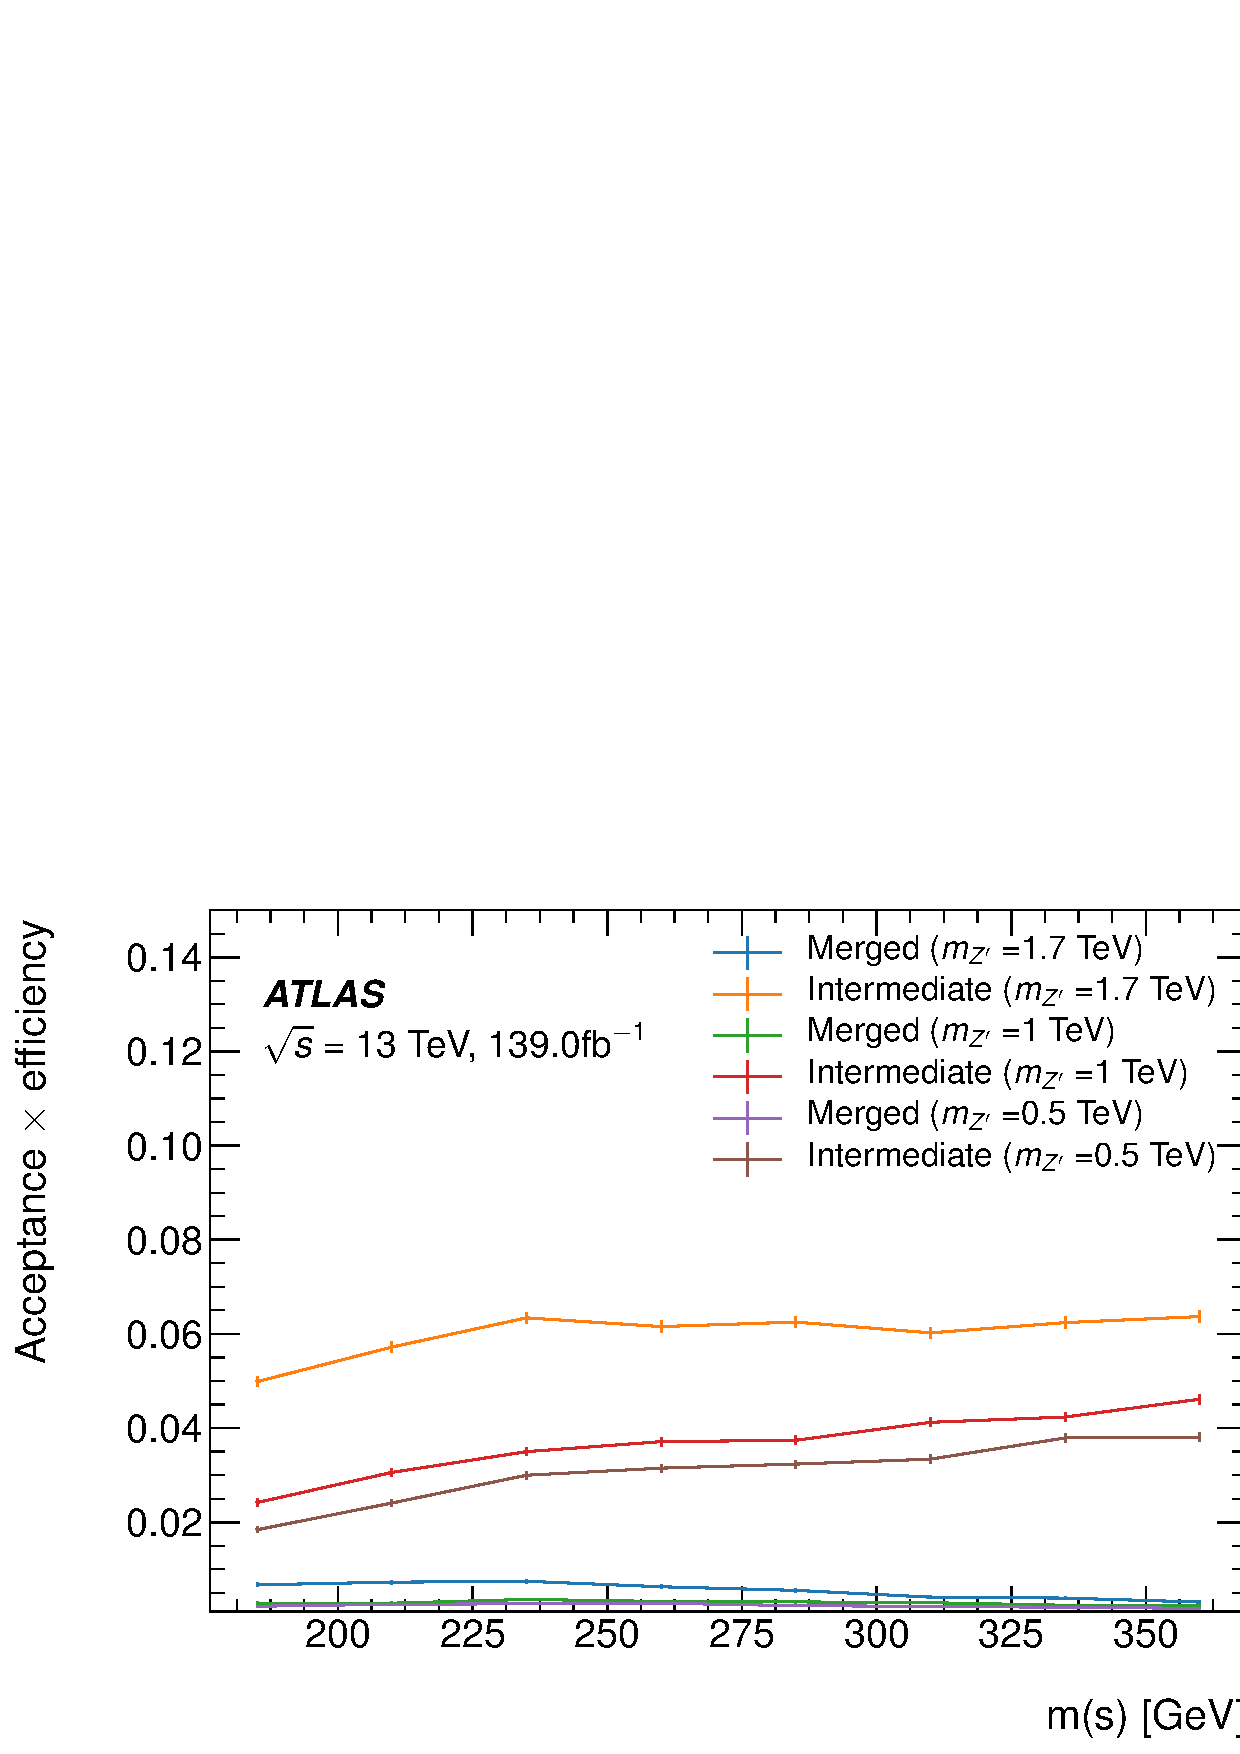
\includegraphics[width=1.\textwidth]{figures/monoS/accXeff_zz.pdf}
    \caption{(\(\mathcal{A} \times \varepsilon\)) for \HepProcess{s \to \PZ \PZ} signal processes.}
  \end{subfigure}
  \caption{The product of detector acceptance and selection efficiency (\(\mathcal{A} \times \varepsilon\)) for the \HepProcess{s \to \PW \PW} (top) and \HepProcess{s \to \PZ \PZ} (bottom) signal processes with the \PZprime boson mass \(\mZp = \SI{0.5}{\tera\electronvolt}, \SI{1}{\tera\electronvolt}, \SI{1.7}{\tera\electronvolt}\), shown in dependence on the dark Higgs boson mass \ms. The points are connected in order to guide the eye.}
  \label{fig:monoSVV:selection:sr:accXeff}
\end{figure}



\section{Background estimation}
\label{sec:monoSVV:backgrounds}
The estimation of the dominant background processes in the \(\met + \sVV\) search is improved by control region data. The CR event selections are defined by requirements on the lepton multiplicity and therefore do not overlap with the SR selection. The CRs have a high purity in the specific background processes. In contrast to the signal process, the dominant background processes have no characteristic peak in the dark Higgs boson candidate mass distributions. Therefore, only \metnomu and \ptll information is used.

The normalisation parameters of the sub-dominant background processes are set to their predicted values based on theoretical predictions and can vary within the corresponding uncertainties.

\subsection{1 muon control region}
\label{sec:monoSVV:backgrounds:cr1}
The 1 muon CR is defined to constrain \wjets processes, which can contribute to the SR through inefficiencies in the lepton reconstruction and due to the limited detector acceptance. Consequently, the selected events contain exactly one tight signal muon, no additional baseline muons and no baseline electrons. The variable \metnomu is introduced, which is reconstructed by neglecting muons in the \met calculation. Events in the 1 muon CR are selected by \met triggers.
The selection requirements are identical to those of the SR which are listed in \Cref{tab:monoSVV:selection:sr:overview}, except for the use of \metnomu instead of \met.

\subsection{2 lepton control region}
\label{sec:monoSVV:backgrounds:cr2}
The 2 lepton CR is designed to constrain the \zjets background using leptonically decaying \zjets events. The dilepton transverse momentum \ptll serves as a proxy of the missing transverse momentum.
Events in the 2 lepton CR are selected by single lepton triggers.
The selected events contain  either exactly two baseline electrons \HepProcess{\Pe \Pe} or exactly two baseline muons \HepProcess{\Pgm \Pgm}. At least one of the two electrons must satisfy \(\pt^{\Pe} > \SI{27}{\giga\electronvolt}\). Similarly, at least one of the two muons must satisfy \(\pt^{\Pgm} > \SI{25}{\giga\electronvolt}\) and \(\abs{\eta^{\Pgm}} < 2.5\). Events containing two muons are only selected if these are of opposite charge. A similar requirement is not applied for events containing two electrons due to higher rate of electron charge misidentification.

A requirement on the invariant mass of the dilepton system \(\SI{83}{\giga\electronvolt} < m_{\Pl \Pl} < \SI{99}{\giga\electronvolt}\) ensures high purity in \zjets processes by suppressing backgrounds with a non-resonantly produced lepton-pair.

The selection requirements are otherwise identical to those of the SR which are listed in \Cref{tab:monoSVV:selection:sr:overview}, except for the use of \ptll instead of \met and the absence of the multijet-suppression requirements.

\subsection{Multijet background estimate}
\label{sec:monoSVV:backgrounds:multijet}
The multijet background is negligible in the SR selection due to the stringent multijet-suppression requirements and the \(\met > \SI{200}{\giga\electronvolt}\) requirement. Similarly, its contribution to the CR selection is vanishing due to the additional requirements on leptons.

Based on an MC-based estimation using the simulated \PYTHIA dijet sample, this background is suppressed to a similar order of magnitude as the statistical uncertainty of the observed data or below.
\Cref{fig:monoSVV:selection:backgrounds:multijet:distributions} shows the distributions \(\min \Delta \varphi(\text{jets}_{1,2,3}, \met)\) and the object-based \met significance for the baseline selection without the multijet-suppression requirements applied.

\begin{figure}[hbtp]
  \centering
  \begin{subfigure}{.49\textwidth}
    \centering
    \includegraphics[width=1.\textwidth]{figures/monoS/monoS_SR_Preselection_minDPhi.pdf}
    \caption{\(\min \Delta \varphi(\text{jets}_{1,2,3}, \met)\)}
  \end{subfigure}
  \begin{subfigure}{.49\textwidth}
    \centering
  \includegraphics[width=1.\textwidth]{figures/monoS/monoS_SR_Preselection_metsig.pdf}
    \caption{Object-based \met significance}
  \end{subfigure}
  \caption{Distributions of the \(\min \Delta \varphi(\text{jets}_{1,2,3}, \met)\) (left) and object-based \met significance (right) variables, which define the multijet-suppression requirements, shown for the observed data~(black dots), background processes~(stacked histograms) scaled to their theoretical expectation, and two representative signal processes~(red and blue dashed lines). The multijet background is estimated with MC simulated events.}
  \label{fig:monoSVV:selection:backgrounds:multijet:distributions}
  % python XAMPPplotting/python/DataMCPlots.py -c XAMPPmonoS/data/PlottingConfigs/DSConfigs/MonoS_SR.py --noATLAS --noSyst --noSignalStack -r SR_Prelection_noAntiQCD --LegendTextSize 18 --LegendXCoords 0.55 0.95 --LegendYCoords 0.48 0.9 --doLogY -v event_dPhi_min_MET_jet123  --regionLabel "SR baseline (no anti-QCD)"
  % python XAMPPplotting/python/DataMCPlots.py -c XAMPPmonoS/data/PlottingConfigs/DSConfigs/MonoS_SR.py --noATLAS --noSyst --noSignalStack -r SR_Preselection_noAntiQCD --LegendTextSize 18 --LegendXCoords 0.55 0.95 --LegendYCoords 0.48 0.9 --doLogY  --regionLabel "SR baseline (no anti-QCD)" -v met_significance_noPUJets_noSoftTerm
\end{figure}

The simulated multijet events are rejected by the multijet-suppression requirements and are thus neglected in the statistical model. A rough data-driven estimate is performed to express certainty.

Multijet-enriched selections are defined for the merged and intermediate categories by removing the \(\min \Delta \varphi(\text{jets}_{1,2,3}, \met) > \SI{20}{\degree}\) requirement and modifying the requirement on \met to \(\SI{150}{\giga\electronvolt} < \met < \SI{200}{\giga\electronvolt}\).

In these multijet-enriched selections, a scale factor for the simulation-based multijet event yield is determined as the ratio of the number of multijet events in data to the multijet events in simulation
\begin{align}
    \text{SF}^{\text{multijet}} = \frac{N(\text{data}) - N(\text{other backgrounds})}{N(\text{simulated multijet background})},
\end{align}
where the number of multijet events in data is roughly estimated by subtracting the event yields of the other background processes normalised to their prediction while neglecting uncertainties.
This results in \(\text{SF}^{\text{multijet}}\) of \num{2.24} in the SR merged category and \num{1.44} in the SR intermediate category, respectively. The scale-factors differ from unity because of the various reasons, the most important being imperfections in the description of the multijet background with \LO accuracy in QCD and the notoriously difficult modelling of tails in the jet energy resolution.

The product of the simulation-based multijet event yield and \(\text{SF}^{\text{multijet}}\) provides an upper estimate in the order of magnitude for the contribution of multijet events in the SR. The results of the estimate are shown in \Cref{tab:monoSVV:selection:backgrounds:multijet:results}.

\begin{table}[ht]
\centering
  \caption{Event yields for the simulated multijet background (dijet MC) and their product with the scale factor \(\text{SF}^{\text{multijet}}\) in the SR merged and intermediate categories. The observed data and the corresponding statistical uncertainty are shown in comparison.}
  \label{tab:monoSVV:selection:backgrounds:multijet:results}
  \begin{tabular}{l rr}
  \toprule
  Signal region       & \textbf{Merged}                 & \textbf{Intermediate} \\
  \midrule
   Dijet MC           & \(2.4 \pm 2.4\)  & \(300 \pm 160\) \\
   Scaled dijet MC    & \(5.4 \pm 5.4\)  & \(440 \pm 230\) \\
  \midrule
   Observed data      & \(825 \pm 29\)   & \(80519 \pm 280\) \\
  \bottomrule
  \end{tabular}
\end{table}

\section{Systematic uncertainties}
\label{sec:monoSVV:systematics}
Systematic uncertainties arise from biases in the reconstruction of compound physics objects and the description of the signal and background processes using MC simulation.

\subsection{Experimental systematic uncertainties}
\label{sec:monoSVV:systematics:experimental}
The experimental systematic uncertainties in the \(\met + \sVV\) search due to biases in the reconstruction of physics objects resemble those of the \(\met + \Hbb\) search. The uncertainties which are similar pertain to the trigger, the pile-up modelling, the reconstruction and calibration of electrons, muons, small-radius jets, \btagging, and the \met reconstruction. The differences in the experimental uncertainties between the two searches are listed below.

\begin{itemize}
  \item \textbf{Luminosity.} The uncertainty on the measurement of the integrated luminosity is \SI{1.7}{\percent}~\cite{ATLAS-CONF-2019-021}.
  \item \textbf{Large-radius jets.} No uncertainties on large-radius jets are considered, as TAR jets are used instead to reconstruct the dark Higgs boson candidates.
  \item \textbf{Small-radius jets.} The calibration of small-radius jets is subject to multiple sources of uncertainty~\cite{PERF-2016-04}. In total, the uncertainties on the JES calibration are parametrised by over 125 components. These components are grouped into a reduced set of 30 components which are derived from the in-situ calibration, pile-up effects, the jet-flavour dependence, and other effects. The JER uncertainties are described by a set of 8 components which are derived from the in-situ calibration.
  \item \textbf{Tracking.} The track reconstruction systematic uncertainties describe the residual alignment uncertainties in the impact parameters \(d_{0}\) and \(z_{0}\), the impact parameter resolution, uncertainties on the tracking efficiency and on the track fake rate and a dedicated uncertainty for tracking in dense environments~\cite{ATL-PHYS-PUB-2015-051}. These systematic uncertainties are parametrised by 12 components.
\end{itemize}

\subsection{Theoretical systematic uncertainties}
\label{sec:monoSVV:systematics:theoretical}
The theoretical systematic uncertainties arise from the description of the signal and background processes, in which the specific choices of event generators, PDF sets, parton shower modelling, and values of the renormalisation and factorisation scales can introduce systematic biases.

The total normalisations of the dominant background processes \zjets and \wjets are constrained by the control region data.
The normalisations of the sub-dominant background processes are constrained by the theoretical normalisation uncertainties, which are listed in \Cref{tab:monosVV:systematics:theoretical:norm}.

\begin{table}[hbtp]
\caption{Theoretical systematic uncertainties on the normalisation of background processes in the \(\met + \sVV\) search.}
\label{tab:monosVV:systematics:theoretical:norm}
\centering
\begin{tabular}{l r}
\toprule
\textbf{Process} & \textbf{Uncertainty} \\
\midrule
\ttbar & \SI{5}{\percent} \\
Single top quark (\(s\)-channel) & \SI{4.6}{\percent} \\
Single top quark (\(t\)-channel) & \SI{4.4}{\percent} \\
Single top quark (\(\PW t\)-process) & \SI{6.2}{\percent} \\
\midrule
\HepProcess{\PW \PW} & \SI{25}{\percent} \\
\HepProcess{\PW \PZ} & \SI{26}{\percent} \\
\HepProcess{\PZ \PZ} & \SI{20}{\percent} \\
\VHbb & \SI{30}{\percent} \\
\bottomrule
\end{tabular}
\end{table}

In addition, shape uncertainties on the dark Higgs boson candidate mass and \met distributions are considered for the dominant background processes, as well as acceptance uncertainties which account for the migration of events among the merged and intermediate categories.
The \met shape uncertainty allows for relative changes in the event yield in the two merged category \met bins, leaving the total event yield unchanged. Similarly, the acceptance uncertainties allow for relative variations in the population of merged and intermediate categories, keeping the event yield sum of both categories constant.
These uncertainties are obtained by comparing samples simulated with different event generator settings.

In contrast to the other searches discussed in this dissertation, the uncertainties are evaluated with simulated samples considering the full detector simulation. The stringent TAR jet substructure requirements applied in the event selection have no equivalent description on particle level. Therefore, the evaluation of the theoretical systematic uncertainties on particle level is not possible.

Three sources of theoretical systematic uncertainty are considered for the dominant \vjets background processes, which are listed below.
\begin{itemize}
  \item The \textbf{scale} uncertainties are estimated by varying the renormalisation scale \muR and factorisation scale \muF coherently by factors of \num{0.5} and \num{2} on an event-by-event basis. The largest variation with respect to the nominal value is taken as the scale uncertainty.
  \item The \textbf{PDF} uncertainty is estimated using the set of 100 eigen-variations of the \textsc{NNPDF30NLO} PDF set~\cite{Ball2015} via the standard deviation approach, in which the uncertainty is computed as
  \begin{align}
    \Delta X = \sqrt{\frac{1}{N-1} \sum_{i=1}^{N} (X_{i} - X_{0})^2}.
  \end{align}
Here, \(N=100\) is the number of PDF replicas, \(X_{i}\) is the event yield for the \(i\)-th PDF variation, and \(X_{0}\) is the mean value of the event yield over all PDF variations. It is added in quadrature with variations of the coupling strength of the strong interaction \(\Delta \alpha_{s} = \pm 0.01\), following the \textsc{PDF4LHC} recommendations~\cite{Butterworth:2015oua}.
  \item The uncertainties related to the choices of \textbf{event generator} and \textbf{parton shower + hadronisation} model are evaluated using alternative MC samples. These are generated with \MGMCatNLOV{2.6.2} at \LO with up to four final-state partons using the \textsc{NNPDF23LO} PDF set and interfaced to \PYTHIAV{8.230}. The CKKW-L merging procedure~\cite{Lnnblad2002,Lnnblad2012} is used with a matching scale of \SI{30}{\giga\electronvolt} to remove the overlap in the description of final-state partons by the hard scattering and the parton shower modelling. As the uncertainties on the \(m_{VV}\) shape are subject to large statistical fluctuations, the distributions were smoothed by cubic spline fits.
\end{itemize}

The average size of the \(m_{VV}\) shape uncertainties is in the range \SIrange{1}{20}{\percent}, with the largest uncertainty coming from the scale variations and the choice of the event generator and the parton shower + hadronisation model.


The theoretical uncertainties for the dark matter signals in the 2MDM model are estimated by variations in the event generation, considering two sources of uncertainty which are listed below.
\begin{itemize}
  \item The \textbf{scale} uncertainties are estimated by varying the renormalisation scale \muR and factorisation scale \muF coherently by factors of \num{0.5} and \num{2} on an event-by-event basis. The largest variation with respect to the nominal value is taken as the scale uncertainty.
  \item The \textbf{PDF} uncertainty is estimated using the standard deviation approach described above, except that no variations of the strong coupling are considered.
\end{itemize}

The average size of the signal uncertainties due to scale variations is of the order of \SI{10}{\percent}, while the PDF uncertainties are typically smaller with values in the range of \SIrange{3}{4}{\percent}.


\section{Statistical model}
\label{sec:monoSVV:model}
The statistical model is based on the likelihood function \Cref{eq:methods:statistics:likelihood}. The profile likelihood fit is based on the invariant mass of the dark Higgs boson candidate in the three SR categories based on \met and the event topology. In the 1 muon CR and the 2 lepton CR, it is based on the event yield in similar categories, which are defined by \metnomu and \ptll, respectively.
A summary of all regions and kinematic distributions considered in the statistical model is provided in \Cref{tab:monoSVV:model:overview}.

\begin{table}[hbtp]
\caption{Summary of all regions and kinematic distributions considered in the statistical analysis of the \(\met + \sVV\) search.}
\label{tab:monoSVV:model:overview}
\centering
\resizebox{1.\textwidth}{!}{%
\begin{tabular}{cccc}
\toprule
& \textbf{0 leptons} & \textbf{1 muon} & \textbf{2 leptons} \\
\midrule
Process of interest & signal & \wjets & \zjets \\
\midrule
Primary fitted observable & \(m_{VV}\)& event yield & event yield \\
Auxiliary fitted observable & \met & \metnomu & \ptll \\
\multirow{2}{*}{Binning} & \multicolumn{3}{l}{merged category: \SIrange{300}{500}{\giga\electronvolt}, \SI{500}{\giga\electronvolt} or more} \\
& \multicolumn{3}{l}{intermediate category: \SI{200}{\giga\electronvolt} or more} \\
\bottomrule
\end{tabular}%
}
\end{table}

\section{Results}
\label{sec:monoSVV:results}
The results of the \(\met + \sVV\) search are presented in this section.
The observed results are presented in \Cref{sec:monoSVV:results:observed}. The impact of groups of systematic uncertainty on the sensitivity of the search is discussed in \Cref{sec:monoSVV:results:impact}.  Finally, the results are interpreted to constrain the parameter space of the 2MDM simplified model in \Cref{sec:monoSVV:results:limits-2mdm}.

\subsection{Observed results}
\label{sec:monoSVV:results:observed}
The background description by the statistical model is validated by performing a conditional background-only (\(\mu = 0\)) fit and investigating the corresponding distributions in the CRs.

\Cref{fig:monoSVV:results:observed:cr1} and \Cref{fig:monoSVV:results:observed:cr2} show the dark Higgs boson candidate mass distributions in the 1 muon CR and in the 2 lepton CR, respectively.
Although only the CR event yield is used in the statistical analysis, the mass distributions are shown to demonstrate adequate modelling in the merged and intermediate categories.
The observed data in the CRs are in good agreement with the SM background prediction, thereby validating the background description.

\begin{figure}[htbp]
\centering
  \begin{subfigure}{1.\textwidth}
    \centering
    \includegraphics[width=.7\textwidth]{figures/monoS/postfit/paper_merged500_1lep_mVV_XS.pdf}
    \caption{1 muon CR merged category \(\metnomu > \SI{500}{\giga\electronvolt}\)}
  \end{subfigure}
  \\
  \begin{subfigure}{1.\textwidth}
    \centering
    \includegraphics[width=.7\textwidth]{figures/monoS/postfit/paper_merged300500_1lep_mVV_XS.pdf}
    \caption{1 muon CR merged category \(\SI{300}{\giga\electronvolt} < \metnomu < \SI{500}{\giga\electronvolt}\)}
  \end{subfigure}
  \\
  \begin{subfigure}{1.\textwidth}
    \centering
    \includegraphics[width=.7\textwidth]{figures/monoS/postfit/paper_intermediate_1lep_mVV_XS.pdf}
    \caption{1 muon CR intermediate category \(\metnomu > \SI{200}{\giga\electronvolt}\)}
  \end{subfigure}
  \caption{Distributions of the dark Higgs boson candidate invariant mass in the 1 muon CR merged and intermediate categories after the background-only fit to the data. The upper panel shows the comparison of data to the SM background expectation before~(dashed lines) and after the background-only fit~(solid histograms). The lower panels display the ratio of data to SM expectations after the fit, with the hatched band expressing the systematic uncertainty. No \(m_{VV}\) shape information in the CRs is considered in the fit.}
  \label{fig:monoSVV:results:observed:cr1}
\end{figure}

\begin{figure}[htbp]
\centering
  \begin{subfigure}{1.\textwidth}
    \centering
    \includegraphics[width=.7\textwidth]{figures/monoS/postfit/paper_merged500_2lep_mVV_XS.pdf}
    \caption{2 lepton CR merged category \(\metnomu > \SI{500}{\giga\electronvolt}\)}
  \end{subfigure}
  \\
  \begin{subfigure}{1.\textwidth}
    \centering
    \includegraphics[width=.7\textwidth]{figures/monoS/postfit/paper_merged300500_2lep_mVV_XS.pdf}
    \caption{2 lepton CR merged category \(\SI{300}{\giga\electronvolt} < \metnomu < \SI{500}{\giga\electronvolt}\)}
  \end{subfigure}
  \\
  \begin{subfigure}{1.\textwidth}
    \centering
    \includegraphics[width=.7\textwidth]{figures/monoS/postfit/paper_intermediate_2lep_mVV_XS.pdf}
    \caption{2 lepton CR intermediate category \(\metnomu > \SI{200}{\giga\electronvolt}\)}
  \end{subfigure}
  \caption{Distributions of the dark Higgs boson candidate invariant mass in the 2 lepton CR merged and intermediate categories after the background-only fit to the data. The upper panel shows the comparison of data to the SM background expectation before~(dashed lines) and after the background-only fit~(solid histograms). The lower panels display the ratio of data to SM expectations after the fit, with the hatched band expressing the systematic uncertainty. No \(m_{VV}\) shape information in the CRs is considered in the fit.}
  \label{fig:monoSVV:results:observed:cr2}
\end{figure}

The results of the profile likelihood fit of the statistical model to the data are reported in terms of the discovery significance for 2MDM simplified model signals in dependence of \mZp and \ms in \Cref{tab:monoSVV:results:results:observed:significance}.

\begin{figure}[htbp]
\centering
  \begin{subfigure}{1.\textwidth}
    \centering
    \includegraphics[width=0.85\textwidth]{figures/monoS/monoS-2mdm-significances_expected.pdf}
    \caption{Expected median discovery significance}
  \end{subfigure}
  \\
  \begin{subfigure}{1.\textwidth}
    \centering
    \includegraphics[width=0.85\textwidth]{figures/monoS/monoS-2mdm-significances_observed.pdf}
    \caption{Observed discovery significance}
  \end{subfigure}
  \caption{Expected median discovery significance \(Z^{\text{exp}}\)~(top) estimated with the Asimov dataset generated under the assumption of the nominal signal model (\(\mu=1\)) and observed discovery significance~(bottom) for the 2MDM simplified model signals in dependence of the \PZprime mediator mass \mZp and the dark Higgs boson mass \ms.}
  \label{tab:monoSVV:results:results:observed:significance}
\end{figure}

No significant deviations from the background-only hypothesis have been observed. Therefore, the results in the SR are presented with the background normalisations scaled to the outcome of the conditional background-only (\(\mu = 0\)) fit.

The observed number of events in the SR event selection for each category is shown in \Cref{tab:monoSVV:results:observed:yield}, together with the expected number of events for the individual background processes, whose normalisation is determined by the background-only profile likelihood fit.

\begin{table}[hbtp]
\caption{Expected and observed numbers of events in the merged event topology signal region with an integrated luminosity of \SI{139}{\per\femto\barn} and \(\sqrt{s} = \SI{13}{\giga\electronvolt}\). The background yields and uncertainties are shown after the profile-likelihood fit to the data. The quoted background uncertainties include both the statistical and systematic contributions.}
\label{tab:monoSVV:results:observed:yield}
\centering
\sisetup{round-mode=figures, round-precision=2,
         retain-explicit-plus=true, group-digits=integer, group-minimum-digits=4}
\begin{tabular}{l%
S[table-format=3.1, table-number-alignment=right, round-mode=figures, round-precision=3]@{$\,\pm\,$}
S[table-format=2.1, table-number-alignment=right, round-mode=figures, round-precision=2]@{\quad}
S[table-format=3.1, table-number-alignment=right, round-mode=figures, round-precision=3]@{$\,\pm\,$}
S[table-format=2.1, table-number-alignment=right, round-mode=figures, round-precision=2]@{\quad}
S[table-format=5.1, table-number-alignment=right, round-mode=figures, round-precision=3]@{$\,\pm\,$}
S[table-format=3.1, table-number-alignment=right, round-mode=figures, round-precision=2]@{\quad}}
\toprule
\multirow{2}{*}{Process} & \multicolumn{6}{c}{Range in \met [\si{\giga\electronvolt}]} \\
& \multicolumn{2}{c}{merged \([300,500)\)} & \multicolumn{2}{c}{merged \([500,\infty)\)} & \multicolumn{2}{c}{intermediate\([200,\infty)\)} \\
\midrule
\zjets & 384 & 27 & 117 & 10 & 49067 & 717 \\
\wjets & 185 & 20 & 24 & 6 & 25453 & 795 \\
\ttbar & 40 & 9 & 7 & 5 & 2533 & 395 \\
Single top-quark & 5 & 3 & 1 & 1 & 631 & 89 \\
Diboson & 38 & 8 & 11 & 3 & 2807 & 454 \\
\midrule
Bkg & 653 & 23 & 160 & 11 & 80497 & 287 \\
Data & \multicolumn{2}{l}{\dat{647}} & \multicolumn{2}{@{}l}{\dat{178}} & \multicolumn{2}{@{}l}{\dat{80519}}  \\
\bottomrule
\end{tabular}
\end{table}

The overall event yields in the CRs and the SR are shown in \Cref{fig:monoSVV:results:observed:summary}. They are found to be well described by SM processes within uncertainties. In particular, the \metnomu and \ptll shape information of the \wjets and \zjets backgrounds provided by the CRs are propagated to the SR.

\begin{figure}[htbp]
\centering
\includegraphics[width=0.95\textwidth]{figures/monoS/postfit/prelim_SR_CR_postfit_plot.pdf}
\caption{Data and SM background post-fit yields stacked in each SR and CR category with the maximum likelihood estimators set to the conditional values of the combined signal and control region fit. The hatched uncertainty band includes simulation statistical uncertainties, experimental systematic uncertainties, and \vjets theory modelling systematic uncertainties. The red line in the lower panel shows the ratio of the pre-fit to the post-fit background prediction.}
  \label{fig:monoSVV:results:observed:summary}
\end{figure}

The dark Higgs boson candidate mass distributions in the SR are shown in \Cref{fig:monoSVV:results:observed:sr}. The signal process is characterised by a large mass peak, which is most evident in the merged category with \(\met > \SI{500}{\giga\electronvolt}\) due to the relatively low contribution of background processes.
The observed results indicate that the data are overall well described by SM predictions.
A mild excess in data around \(m_{VV} = \SI{160}{\giga\electronvolt}\) is observed. The excess corresponds to a local significance of \(2.3\sigma\) and a global significance of \(1.3\sigma\) when considering the nine independent \ms hypotheses under consideration. Although the excess seems to be most prominent in the intermediate category, it is narrower than the experimental resolution for \ms in this category.

\begin{figure}[htbp]
\centering
  \begin{subfigure}{1.\textwidth}
    \centering
    \includegraphics[width=.7\textwidth]{figures/monoS/postfit/paper_merged500_0lep_mVV_XS.pdf}
    \caption{SR merged category \(\metnomu > \SI{500}{\giga\electronvolt}\)}
  \end{subfigure}
  \\
  \begin{subfigure}{1.\textwidth}
    \centering
    \includegraphics[width=.7\textwidth]{figures/monoS/postfit/paper_merged300500_0lep_mVV_XS.pdf}
    \caption{SR merged category \(\SI{300}{\giga\electronvolt} < \metnomu < \SI{500}{\giga\electronvolt}\)}
  \end{subfigure}
  \\
  \begin{subfigure}{1.\textwidth}
    \centering
    \includegraphics[width=.7\textwidth]{figures/monoS/postfit/paper_intermediate_0lep_mVV_XS.pdf}
    \caption{SR intermediate category \(\metnomu > \SI{200}{\giga\electronvolt}\)}
  \end{subfigure}
  \caption{Distributions of the dark Higgs boson candidate invariant mass in the SR merged and intermediate categories, after the background-only fit to the data. The upper panel shows the comparison of data to the SM background expectation before~(dashed lines) and after the background-only fit~(solid histograms). The lower panels display the ratio of data to SM expectations after the fit, with the hatched band expressing the systematic uncertainty. A representative 2MDM simplified model signal with \(\mZp = \SI{1}{\tera\electronvolt}\), \(\ms = \SI{160}{\giga\electronvolt}\), \(\gq = 0.25\), \(\gchi = 1\), and \(\mchi = \SI{200}{\giga\electronvolt}\) is overlaid.}
  \label{fig:monoSVV:results:observed:sr}
\end{figure}


\subsection{Impact of systematic uncertainties}
\label{sec:monoSVV:results:impact}
The impact of the various sources of systematic uncertainty on the fitted signal strength \(\mu\) is evaluated using the procedure presented in \Cref{sec:monoV:results:impact}.

\Cref{tab:monoSVV:results:impact:breakdown} shows a breakdown of the expected signal strength uncertainties for three representative 2MDM simplified model signals with different \ms. The three 2MDM scenarios are chosen to represent different event topologies. The first signal corresponds to events selected primarily in the merged category, while the third signal corresponds to events selected primarily in the intermediate category. The second signal corresponds to events selected by both categories.

The dominant sources of experimental uncertainty arise from the scale and resolution of the energy of jets, tracking efficiencies, as well as the calibration of the lepton identification. Dominant theoretical systematic uncertainties originate from the modelling of the signal and the \wjets and \zjets background processes, which encompass uncertainties from the choice of PDFs and factorisation and renormalisation scales. Other large systematic uncertainties arise from the statistical uncertainty of the MC simulated events.

As systematic uncertainties dominate the search, a future iteration would strongly benefit from improvements in the jet energy calibration and an improved description of the background processes.

\begin{table}[hbtp]
\caption{Breakdown of expected signal strength uncertainties for three representative 2MDM signal samples with \(\mZp = \SI{1}{\tera\electronvolt}\) and (a)~\(\ms = \SI{160}{\giga\electronvolt}\), (b)~\(\ms = \SI{235}{\giga\electronvolt}\), and (c)~\(\ms = \SI{310}{\giga\electronvolt}\). The effect is expressed as the relative uncertainty on the signal strength, assuming total cross-sections of (a)~\SI{214}{\femto\barn}, (b)~\SI{53}{\femto\barn}~fb, and (c)~\SI{19}{\femto\barn}. Each systematic uncertainty contribution is provided as the quadratic difference between the total uncertainty and the uncertainty obtained by setting the systematic uncertainty in question to its nominal value and excluding it thereby from the fit. Total denotes the quadrature sum of statistical and total systematic uncertainties.}
\label{tab:monoSVV:results:impact:breakdown}
\centering
\begin{tabular}{l rrr}
\toprule
Source & \multicolumn{3}{c}{Uncertainty on \(\mu\) [\si{\percent}]} \\
of uncertainty & (a) & (b) & (c) \\
\midrule
Signal modelling               & 11  & 10  & 10  \\
\wjets modelling               &  9  & 21  & 14  \\
\zjets modelling               &  7  & 12  & 13  \\
Diboson modelling              & 1.1 & 1.0 & 1.5 \\
\ttbar / single \Pqt modelling & 0.3 & 0.5 & 0.7 \\
Pile-up modelling              & 0.2 & 1.1 & 2.3 \\
MC statistics                  & 11  & 14  & 23  \\
\met                           & 5.2 & 0.6 & 2.1 \\
Jet energy scale               & 8   & 17  & 24  \\
Jet energy resolution          & 11  & 18  & 15  \\
Lepton reconstruction          &  8  &  9  & 5   \\
Flavour tagging                & 1.3 & 1.7 & 8.5 \\
Track reconstruction           &  6  &  7  & 5   \\
Luminosity                     & 1.6 & 2.0 & 1.3 \\
\midrule
Systematic uncertainty         & 30 & 42 & 55 \\
Statistical uncertainty        & 16 & 25 & 50 \\
Total uncertainty              & 34 & 49 & 74 \\
\bottomrule
\end{tabular}
\end{table}


\subsection{Constraints on the 2MDM simplified model}
\label{sec:monoSVV:results:limits-2mdm}
As no large deviation from the SM background expectation is observed for any of the signal mass points, the parameter space of the 2MDM simplified model can be constrained by computing upper limits on the signal strength \(\mu\) at \SI{95}{\percent} confidence level using the \(\text{CL}_{s}\) method~\cite{Read:2002hq}.

\Cref{fig:monoSVV:results:limits-2mdm:limits-ms} shows the exclusion limits on the signal strength \(\mu\) for signals in the 2MDM simplified model with \(\mZp = \SI{0.5}{\tera\electronvolt}\), \(\mZp = \SI{1.0}{\tera\electronvolt}\), and \(\mZp = \SI{1.7}{\tera\electronvolt}\) in dependence of \ms.

\begin{figure}[htbp]
\centering
  \begin{subfigure}{1.\textwidth}
    \centering
    \includegraphics[width=.7\textwidth]{figures/monoS/limits/prelim_ms_limits_exp_obs_mZp_500.pdf}
    \caption{Exclusion limits for 2MDM signals with \(\mZp = \SI{0.5}{\tera\electronvolt}\)}
  \end{subfigure}
  \\
  \begin{subfigure}{1.\textwidth}
    \centering
    \includegraphics[width=.7\textwidth]{figures/monoS/limits/prelim_ms_limits_exp_obs_mZp_1000.pdf}
    \caption{Exclusion limits for 2MDM signals with \(\mZp = \SI{1.0}{\tera\electronvolt}\)}
  \end{subfigure}
  \\
  \begin{subfigure}{1.\textwidth}
    \centering
    \includegraphics[width=.7\textwidth]{figures/monoS/limits/prelim_ms_limits_exp_obs_mZp_1700.pdf}
    \caption{Exclusion limits for 2MDM signals with \(\mZp = \SI{1.7}{\tera\electronvolt}\)}
  \end{subfigure}
  \caption{Upper \SI{95}{\percent} \(\text{CL}_{s}\) limits on the signal strength \(\mu\) of 2MDM simplified model signals in dependence of the dark Higgs boson mass \ms for the fixed set of parameters \(\gq = 0.25\), \(\gchi = 1\), and \(\mchi = \SI{200}{\giga\electronvolt}\) in the scenarios with \PZprime boson mediator masses \(\mZp = \SI{0.5}{\tera\electronvolt}\)~(top), \(\mZp = \SI{1.0}{\tera\electronvolt}\)~(middle), and \(\mZp = \SI{1.7}{\tera\electronvolt}\)~(bottom). The observed limits~(solid line) are consistent with the expectation under the background-only hypothesis~(dashed line) within the uncertainties~(filled band), except for a small excess at \(\ms = \SI{160}{\giga\electronvolt}\).}
  \label{fig:monoSVV:results:limits-2mdm:limits-ms}
\end{figure}


The corresponding exclusion limit contour, which is provided in the \mZp-\ms plane for the fixed set of parameters \(\gq = 0.25\), \(\gchi = 1\), and \(\mchi = \SI{200}{\giga\electronvolt}\), is shown in \Cref{fig:monoSVV:results:limits-2mdm:contour}.
The signal points in the 2MDM simplified model with \mZp of up to \SI{1.6}{\tera\electronvolt} are excluded at \SI{95}{\percent} \(\text{CL}_{s}\) for \(\ms = \SI{210}{\giga\electronvolt}\). The observed exclusion range in \mZp becomes narrower than expected at low \ms owing to the small excess in data close to \(m_{VV} = \SI{160}{\giga\electronvolt}\) as discussed above.

\begin{figure}[htbp]
    \centering
    \includegraphics[width=.95\textwidth]{figures/monoS/prelim_limit_contour_monoSvv.pdf}
    \caption{Exclusion contours at \SI{95}{\percent} \(\text{CL}_{s}\) for the 2MDM simplified model in the \mZp-\ms plane for the fixed set of parameters \(\gq = 0.25\), \(\gchi = 1\), and \(\mchi = \SI{200}{\giga\electronvolt}\). The observed limits are encircled by the solid line, whereas the expected limits are indicated by the dashed line.  The expected \(\pm1\sigma\) and \(\pm2\sigma\) uncertainties are shown as filled green and yellow bands. The observed value of the relic density from the Planck~\cite{Planck2020} measurements is obtained for \(\mZp = \SI{850}{\giga\electronvolt}\) (dotted line). The region on the right of the line corresponds to higher predicted relic density than these measurements.}
    \label{fig:monoSVV:results:limits-2mdm:contour}
\end{figure}

\section{Conclusion of the \(\met + \sVV\) search}
\label{sec:monoSVV:conclusion}
In conclusion, the signature of \met and resonant production of weak vector boson pairs is explored for the first time at the LHC. The novelty of TAR jets is applied in this search to reconstruct dark Higgs boson candidates in dense event topologies using \stoVV decays. The TAR jet algorithm improves the sensitivity of the search by a factor of up to 2.5 regarding the expected median discovery significance compared to the conventional large-R jet approach,
assuming similar impact of the systematic uncertainties as suggested by the comparison of \Cref{tab:monoV:results:impact:breakdown} and \Cref{tab:monoSVV:results:impact:breakdown}.

The minor excess invites further investigation, for instance by searches targeting the (semi-)leptonic decay channel of the weak vector bosons.
The 2MDM model can be further explored in the various decay modes of the dark Higgs boson.
Heavy dark Higgs bosons decay to pairs of SM Higgs bosons, which can be probed using the \(\met + \Ph(\Pqb\Paqb) \Ph(\Pqb\Paqb)\) signature.
Very light dark Higgs bosons can be searched for using the \(\met + s(\Pqb\Paqb)\) signature, which awaits further exploration for \(\ms < \SI{50}{\giga\electronvolt}\).
